\section{Architectural Design and Technical Considerations}
\label{sec:architectural_design}
\subsection{Core Principles}


\subsubsection{Fidelity through Clang}
Generating accurate bindings without writing many platform- and language dialect specific details requires a high-fidelity parser for the C language. While various tools exist, a comparative analysis presented in \autoref{app:c_ast_introspection_tools} reveals that leveraging the Clang compiler front-end is the most robust and flexible approach, as Clang is architected to handle various C dialects and emit ABI-compatible code for all major compilers and platforms.

\subsubsection{Safety and Portability through Abstraction}
A source of bugs and unexpected incompatibilities stems from languages importing the platform-dependent C types, like \texttt{long} to a simple type alias to a fixed-width integer type (e.g. \texttt{Int64}) on the target platform using conditional compilation. This approach forces no consideration for platforms where the size may differ, leading to fragile code. To counter this, Hylo's architecture is founded on the principle of abstraction: platform-dependent C types are imported as distinct, non-aliasing types within Hylo (e.g., \texttt{CLong}). These types cannot be used directly in arithmetic with Hylo's fixed-width integers; they require explicit, \textbf{intention-revealing conversions} that force the developer to handle potential narrowing and signedness differences. This design choice makes portability risks visible at the type level, preventing entire classes of errors.

\subsubsection{Idiomatic Hylo through Customization}
A rigid, one-size-fits-all mapping is insufficient because C often uses a single syntactic construct to represent multiple semantic ideas. A C enum, for example, could be a set of mutually exclusive cases, a collection of combinable bitflags, or simply a group of named constants. Thus, Hylo must empower developers to map these C idioms to the most appropriate and type-safe construct for ergonomic experience.

This principle is realized through a framework of sensible defaults with developer-driven customization, for which the system provides two primary mechanisms:
\begin{itemize}
    \item \textbf{Rule Files:} External configuration files allow developers to specify mapping rules for C headers they do not own, enabling non-intrusive customization for system libraries or third-party dependencies. Rules can be applied globally, per-header, or use name-based pattern matching. Flexibility of domain-specific languages is often limited, thus we recommend adopting regular Hylo code for specifying the importing rules, with a library of helper primitives.
    \item \textbf{In-Source Annotations:} When developers have ownership of the C source, they can use annotations directly in the header files to improve local reasoning and maintainability. Unlike Swift's attribute-based C code annotations that require compiler extensions to work, Hylo shall adopt Bindgen's approach of using comments with HTML tags and attributes to prevent the annotations from being rendered as part of the C documentation by existing tools.
\end{itemize}

\subsection{System Overview}
The two main challenges every native interoperability tool must solve are understanding the memory layout of C data structures and calling C functions with the correct calling convention according to the C application binary interface (ABI). The calling convention defines details such as which parameters to pass in registers or on the stack, how values are returned from a function and what registers are callee or caller saved.

\begin{figure}[]
    \includegraphics[width=1\textwidth]{attachments/architecture-overview.pdf}
    \caption{\textbf{Architecture Overview}: extending the compilation pipeline with an FFI binding generator.}
    \label{fig:architecture}
\end{figure}

As shown in \autoref{fig:architecture}, our design extends Hylo's compilation pipeline with a C binding generator. This tool parses C header files using LibClang, applies developer-defined mapping rules, and emits corresponding .hylo declarations to either files or directly into Hylo abstract syntax tree (AST). The Hylo compiler then processes these generated declarations alongside the rest of the program's source code. Finally, the resulting object files are linked with the necessary C libraries—either statically or at runtime—to produce the final executable. By leveraging LibClang, we can capture the precise memory layout into the generated Hylo structs, while LLVM allows us to call C functions according to the platform's C ABI which are detailed in the following sections.

\subsection{Capturing the Memory Layout: Opaque Storage for Composite Types}
\label{ssec:layout-capture}

C structs and unions are challenging to map to other languages because the new language has to replicate the memory layout of the original type, so that field access is done with correct memory offsets. Determining the struct layout involves handling the size and alignment of members, potentially including padding, and distributing bit-fields. The layout may also be influenced by compiler-specific packing attributes in all major C compilers, though their behavior is consistent.\footnote{See the effect of packing attributes in MSVC, Clang and GCC: \url{https://edu.nl/8hg98}}

C bit-fields have largely implementation-defined layout rules, which can vary significantly between compilers\footnote{See an example of varying layout of bit-fields: \url{https://godbolt.org/z/xqPEvs6YK}}. Due to the challenging nature of C bit-fields, many C interop technologies do not support interoperating with structs with bit-fields\footnote{See \href{https://github.com/rust-lang/rfcs/issues/314}{Rust's open issue about bit-field support in \texttt{\#[repr(C)]}}}\footnote{See Zig's tracking issue \href{https://github.com/ziglang/zig/issues/1499}{\#1499} for implementing bit-field support.}, and it is generally recommended to avoid using them in separately compiled library code, as interoperability is not even guaranteed between C compilers.

We identified two existing approaches for interoperating with bit-fields:

\begin{enumerate}
    \item Rust lets us \textbf{annotate Rust structs, unions and enums --that have C-compatible members--} with the \texttt{\#[repr(C)]} attribute. Rust then lays out these members according to the C ABI by reimplemented logic\cite{rust-c-layouting}. Notably, bit-fields are not supported natively.
    
    However, Bindgen\cite{rust-bindgen}, an external binding generator for Rust, attempts to emit Rust \texttt{\#[repr(C)]} structs from C header files, complementing the layout algorithm with a custom bit-field handling algorithm, and exposing accessor methods that let the user operate with a correctly aligned and padded Rust integer type. This method can often work but has limitations and bugs, a notable problem being that C bit-fields may share storage with other members' padding bits, which is challenging to replicate when generating separate struct fields for each member.\footnote{See \href{https://github.com/rust-lang/rust-bindgen/issues/743\#issuecomment-321051199}{issue \#743 in Bindgen's repository} related to the overlapping storage bug.}.
    
    \item Swift imports C declarations by \textbf{directly embedding Clang into the compiler}, and transforming declarations from Clang AST directly to Swift AST declarations\footnote{See structs being imported to Swift in \href{https://github.com/swiftlang/swift/blob/9a0a831b0198e1b794a66316487aacef3d692ca4/lib/ClangImporter/ImportDecl.cpp\#L2079}{ImportDecl.cpp at line 2079}}. It synthesizes computed properties for accessing C bit-fields, which present an API as if the bit-fields were regular Swift fields while performing the necessary bit-masking and shifting to access the individual fields\cite{how-swift-imports-c-structs}. Swift preserves the references to the original Clang AST nodes, which can be used when compiling member access to find out the exact member offsets, therefore resulting in a robust mapping.
\end{enumerate}

The first approach, decoupling the mapping of implementation-defined C constructs from the main compiler is useful for reducing the compiler's binary size (no need to embed Clang in the general case), simplifies the development environment setup for both the compiler authors and its users, and keeps the bugs easier to fix in the substantially smaller codebase of the binding generator. On the other hand, embedding Clang and directly maintaining layout information from the Clang AST for the backend reduces the maintenance burden of the binding generator, and allows for robust handling of implementation-defined C constructs.

We propose a hybrid approach for Hylo that combines advantages from both methods, shown in \autoref{fig:layout}. Instead of letting the Hylo compiler take care of C struct layout, we map members of unions and structs to a Hylo struct containing a \textbf{contiguous inline byte sequence} with the same length as the original C type's size (including padding bytes). Subsequently, we synthesize computed properties (subscripts) for accessing the individual members, which provide idiomatic access to the members, exactly as if they were stored properties. For struct members, we can leverage LibClang's functions (e.g. \texttt{clang\_Cursor\_getOffsetOfField}) to get the offset, the size in bytes of the underlying type and the bit-width in case of bit-fields. Union members always start a  t the same memory address, without an offset\cite{c23-struct-and-union-specifiers}.
\begin{figure}
    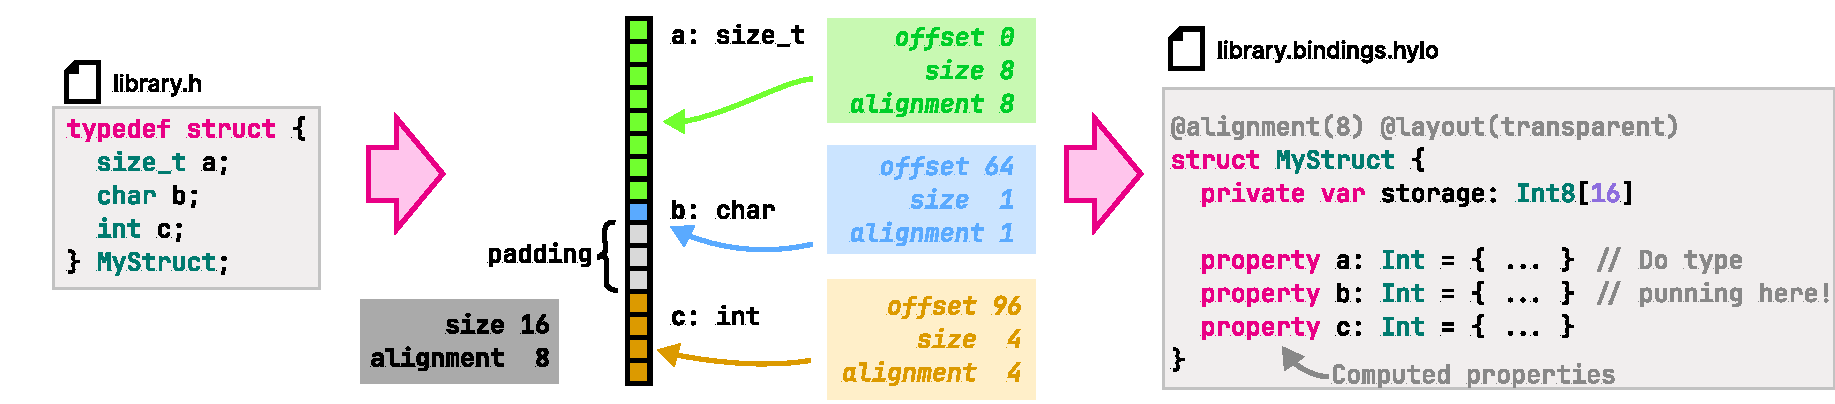
\includegraphics[width=1\textwidth]{attachments/layout.pdf}
    \caption{\textbf{Capturing the Memory Layout of C Constructs}}
    \label{fig:layout}
\end{figure}
To ensure the same data layout in Hylo as in C, we need an additional annotation for the Hylo struct: we need to specify its \textit{alignment}, so that the Hylo compiler can know on which boundary it should allocate instances of the struct.

\subsection{Function Calls}
//// GENERAL CASE
TODO discuss what responsibilities are there to correctly call functions 

//// todo: describe what are the inherent things that need to be different in ABIs based on different architectures, and what are imposed by the OS and the C language. Mention the problem of compilers incorrectly implementing ABIs which sometimes necessitates the interop tool to implement workarounds for specific compilers or platforms (link Emilio interview).

Reimplementing the complex ABI logic for every supported platform is a monumental and error-prone task. Instead, our proposed architecture leverages Clang's own ABI handling capabilities. Since Hylo uses LLVM as its backend, and Clang is also an LLVM-based compiler, we can delegate the responsibility of ABI-correct function lowering to Clang. The interoperability tool can instruct Clang to generate the LLVM Intermediate Representation (IR) for a call to a C function, ensuring that all platform-specific calling conventions and data layout rules are correctly applied. This approach significantly reduces implementation complexity and ensures correctness by relying on the same battle-tested ABI logic used by Clang itself.

\subsubsection{Compiling Header-Defined Functions: \texttt{static}/\texttt{static inline}/\texttt{inline}}
\label{ssec:handling-inline-c-functions}

A significant challenge in C interop is handling functions defined entirely within header files. These functions, declared with the \texttt{static}, \texttt{inline}, or \texttt{static inline} specifiers, lack a stable, externally visible symbol in the object file, making them non-linkable by default. To invoke them from another language, their implementation must be made accessible. Our analysis reveals two primary architectural approaches to this problem:

\textbf{Generating C Wrappers.} This strategy involves creating a new \texttt{.c} source file that contains simple, externally visible wrapper functions for each desired header-defined function. This file is then compiled alongside the original library, and the foreign language binds to the newly created symbols with unique names (e.g., suffixed with \texttt{\_\_wrapper}). Performance recovery via Link-Time Optimization (LTO) is possible but remains unreliable. It requires a shared compiler backend like LLVM, and even then, the inlining is a heuristic optimization that may not be performed.

This technique is employed by Rust's Bindgen, though it currently has (unnecessary) limitations regarding plain \texttt{inline} functions\cite{bindgen-inline-limitation} that we proposed to mitigate in\cite{bindgen-inline-proposal}.

\textbf{Direct LLVM IR Emission:} A more deeply integrated approach, employed by Swift-C interop, is to use Clang as a library to request the compilation of the header-defined function directly into LLVM Intermediate Representation. LLVM IR can then be consumed by the new language's backend, given that it uses LLVM. By operating at the compiler level rather than the linker level, this strategy eliminates the cost of function calls.

For Hylo, a language early in its development, we adopt the wrapper-generation approach. This prioritizes compiler simplicity and avoids a hard dependency on a specific C compiler front-end or a single backend like LLVM, which we consider a prudent trade-off at this stage.

todo: describe the option to add wrapper function (maybe)

\subsubsection{IDE Integration}

A modern language architecture isn't just about the compiler. It encompasses the entire developer experience. A seamless workflow where IDE features like semantic symbol renaming and go-to-definition work across language boundaries is a critical architectural feature that enhances usability.

Our design proposes the creation of a Hylo Language Server that acts as a proxy, coordinating with \texttt{clangd}, the official C/C++ language server for the LLVM project and Hylo's own language server that leverages the Hylo compiler as a library under the hood. This is a standard approach taken by many web technologies, and more relevantly, by Swift's SourceKit-LSP\footnote{See SvelteKit's \href{https://github.com/sveltejs/language-tools/}{Language Tools}, Angular's \href{https://github.com/angular/angular/tree/main/packages/language-service}{Language Service}, and Swift's \href{https://github.com/swiftlang/sourcekit-lsp}{SourceKit-LSP} for examples.}.

\subsection{Customization and Ambiguous Mappings}

A core principle of our design is acknowledging that a single, direct mapping is often insufficient. Many C constructs are used to represent different semantic ideas. A prime example is the C \texttt{enum}. It can represent:
\begin{enumerate}
    \item A set of mutually exclusive cases \(\rightarrow\) translate to a Hylo enum for proper exhaustiveness checking
    \item A collection of independent bitflags \(\rightarrow\) translate to an \texttt{OptionSet} \cite{OptionSet} for easy combination and checking of binary flags.
    \item A simple group of named integer constants. \(\rightarrow\) translate to a Hylo namespace with constants.
\end{enumerate}
A rigid mapping to a single Hylo construct would be un-idiomatic in at least two of these cases. Therefore, our design proposes a system of \textbf{sensible defaults with user-customizable overrides.} By default, an \texttt{enum} might be imported as a struct of static constants, which is always safe. However, the developer can provide an annotation (e.g., in a separate configuration file or directly in the C header if they have ownership) to guide the mapping:

This principle of user-guided mapping extends to other areas, such as specifying that a C function returning an integer error code should be imported as a Hylo function that \texttt{throws}. This empowers developers to create bindings that are not only correct but also safe and highly idiomatic.

% //// TODO describe the rules file vs inline annotations (comments vs attributes)